\documentclass[
%%%%% Styles and Sizes
%10pt,
%11pt,
%12pt,
fancyheadings, % headings with seplines and logo
%
%%%%% Printing, Color and Binding
%a4paper, 
%a5paper,
%twoside, % single sided printout
%oneside, % duplex printout (default)
%% binding correction is used to compensate for the paper lost during binding
%% of the document
%BCOR=0.7cm, % binding correction
%nobcorignoretitle, % do not ignore BCOR for title page
%% the following two options only concern the graphics included by the document
%% class
%grayscaletitle, % keep the title in grayscale
%grayscalebody, % keep the rest of the document in grayscale
%
%%%%% expert options: your mileage may vary
%baseclass=..., % special option to use a different document baseclass
]{stsreprt}

% Information for the Titlepage
\author{Robin Willenbrock}
\title{Static Detection of Data Races in Interrupt-Driven Software Using Reduced Inter-Procedural Control Flow Graphs}
\date{\today}
\subject{Bachelor Thesis}
\professor{}
\advisor{Ulrike Engeln}

\usepackage[utf8]{inputenc}
\usepackage{listings}
\usepackage{amsmath}
\usepackage{xcolor}
% Font and Fontencoding Magic
% FAQ: 
% http://tex.stackexchange.com/questions/664/why-should-i-use-usepackaget1fontenc
% http://en.wikipedia.org/wiki/Computer_Modern
% http://tex.stackexchange.com/questions/1390/latin-modern-vs-cm-super
\usepackage[T1]{fontenc}
\usepackage{lmodern}
%\usepackage{fix-cm}
\lstset{
	language=Python,
	basicstyle=\ttfamily\footnotesize,
	keywordstyle=\color{blue},
	commentstyle=\color{green},
	stringstyle=\color{red},
	numbers=left,
	numberstyle=\tiny\color{gray},
	stepnumber=1,
	numbersep=5pt,
	frame=single,
	breaklines=true,
	showstringspaces=false,
	tabsize=4,
	captionpos=b
}
\usepackage{tikz}
\usetikzlibrary{shapes.geometric, arrows}
\usepackage{caption}
\usepackage{float}
\usepackage[linesnumbered,ruled,vlined]{algorithm2e}

\tikzstyle{startstop} = [rectangle, rounded corners, minimum width=3cm, minimum height=1cm,text centered, draw=black, fill=red!30]
\tikzstyle{process} = [rectangle, minimum width=3cm, minimum height=1cm, text centered, draw=black, fill=orange!30]
\tikzstyle{decision} = [diamond, minimum width=3cm, minimum height=1cm, text centered, draw=black, fill=green!30]
\tikzstyle{arrow} = [thick,->,>=stealth]
\tikzstyle{redarrow} = [thick,->,>=stealth,draw=red]

\begin{document}
\frontmatter
\maketitle
\tableofcontents
\listoffigures{}
\mainmatter{
\chapter{Introduction}



\chapter{Background}

\section{Interrupt-Driven Systems}
An interrupt-driven system is an architecture where the flow of execution is changed by unpredictable events in the system, also known as interrupts. Interrupts can be caused by hardware devices, software conditions, or external signals forcing the processor to suspend the current task to execute an interrupt handler or interrupt service routine (ISR). Interrupt-driven systems are used in real-time operating systems, embedded systems, and generally in systems where timely responses are necessary \cite{wang2020}.

\begin{figure}[H]
	\centering
	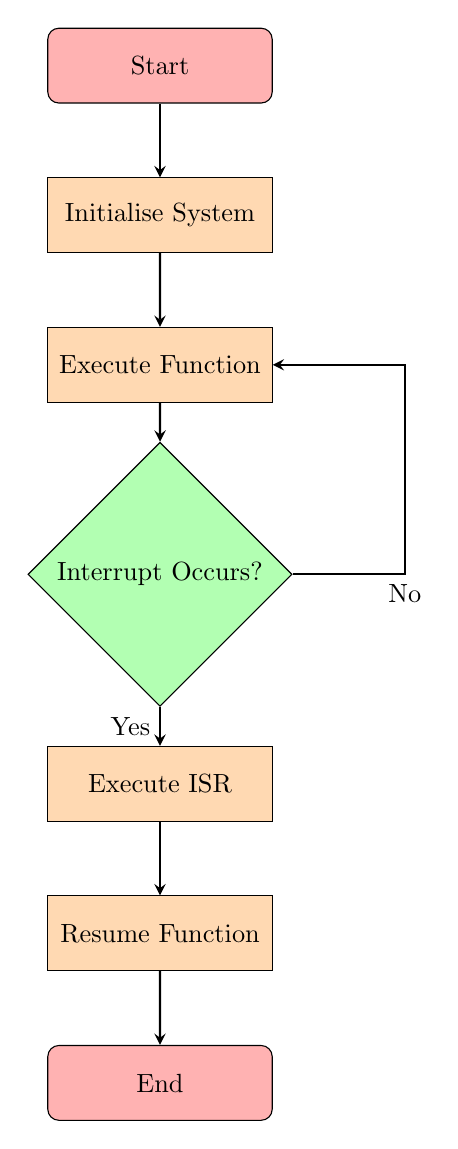
\begin{tikzpicture}[node distance=2cm, scale=0.95, transform shape]
		
		\node (start) [startstop] {Start};
		\node (init) [process, below of=start] {Initialise System};
		\node (exec) [process, below of=init] {Execute Function};
		\node (interrupt) [decision, below of=exec, yshift=-0.8cm] {Interrupt Occurs?};
		\node (isr) [process, below of=interrupt, yshift=-0.8cm] {Execute ISR};
		\node (resume) [process, below of=isr] {Resume Function};
		\node (end) [startstop, below of=resume] {End};
		
		\draw [arrow] (start) -- (init);
		\draw [arrow] (init) -- (exec);
		\draw [arrow] (exec) -- (interrupt);
		\draw [arrow] (interrupt) -- node[anchor=east] {Yes} (isr);
		\draw [arrow] (isr) -- (resume);
		\draw [arrow] (resume) -- (end);
		\draw [arrow] (interrupt.east) -- ++(1.5,0) node[anchor=north] {No} |- (exec.east);
		
	\end{tikzpicture}
	\caption{Flow-Chart des interruptgesteuerten Systems}
\end{figure}

In Figure 2.1, a basic execution flow of a simple interrupt-driven system is displayed. The system executes a function as long as no interrupt occurs. When an interrupt occurs, it switches to the ISR, executes it, and then resumes the function executed before the interrupt happened.

The management of the interrupts to maintain the fast responsiveness of the system is the most challenging part of an interrupt-driven system. Interrupts occur in unpredictable ways, so you have to consider every possible execution flow. To ensure the execution of critical interrupts, interrupts are often prioritised, so higher priority events can interrupt lower ones and be handled immediately. When handling an interrupt, the current state of the processos is saved, and the context is switched to the ISR \cite{wang2020}.

The unpredictivity and asynchronous nature of the interrupts present a lot of challenges in designing and implementing an interrupt-driven system. One of the biggest challenges is the correct handling of high-priority interrupts without delaying them substantially. Which needs a sophisticated scheduling and prioritisation mechanism. The execution of the main programme and ISR needs to be handled properly to ensure data tegrity. Furthermore, handling context switches, preserving system state, and avoiding deadlocks all contribute to the development of an interrupt-driven system.

\section{Shared Resources}
<<<<<<< HEAD
Shared resources are data or hardware components that can be accessed by multiple threads or processes in a concurrent system. These resources include memory locations, files, I/O devices, and communication channels. In interrupt-driven systems, shared resources often involve variables or data structures that are accessed by both the main program and ISRs. Proper management of shared resources is critical to ensure data consistency and avoid conflicts \cite{herlihy2008}.
\subsection{Types of Shared Resources}
\begin{itemize}
	\item \texttt{Memory}: Shared memory locations, such as global variables or heap-allocated data structures, are accessed by multiple threads. Proper synchronization mechanisms, like locks or atomic operations, are required to ensure that memory access is controlled and consistent \cite{herlihy2008}.

	\item \texttt{:I/O Devices}: Hardware devices, such as printers, disk drives, and network interfaces, can be shared among different processes or threads. Access to these devices must be coordinated to prevent conflicts and ensure that operations are performed correctly \cite{burns2009}.

	\item \texttt{Files}: Files on a disk can be accessed by multiple processes. File locks or similar mechanisms are used to manage concurrent access, ensuring that read and write operations do not interfere with each other \cite{labrosse2002}.

	\item \texttt{Communication Channels}: Pipes, message queues, and shared memory segments used for inter-process communication are shared resources that require careful management to avoid data races and ensure the integrity of the communicated data \cite{herlihy2008}
\end{itemize}
\subsection{Managing Shared Resources}
Proper management of shared resources involves the use of synchronization mechanisms to coordinate access and ensure data consistency. Mutexes, semaphores, and condition variables are common tools used to control access to shared resources. Mutexes provide mutual exclusion, ensuring that only one thread can access the resource at a time. Semaphores can limit the number of threads accessing the resource simultaneously. Condition variables allow threads to wait for certain conditions to be met before proceeding, facilitating complex synchronization scenarios \cite{herlihy2008}.

=======
Shared resources, often referred to as shared memory or shared variables, are data that can be accessed simultaneously by multiple threads or processes. Proper management of these resources is crucial because improper handling can lead to issues like data races, deadlocks, and other synchronisation problems. In interrupt-driven systems, shared resources often involve variables or data structures that are accessed by both the main programme and ISRs. Proper management of shared resources is critical to ensuring data consistency and avoiding conflicts \cite{herlihy2008}.
Proper management of shared resources involves the use of synchronisation mechanisms to coordinate access and ensure data consistency. Mutexes, semaphores, and condition variables are common tools used to control access to shared resources. Mutexes provide mutual exclusion, ensuring that only one thread can access the resource at a time. Semaphores can limit the number of threads accessing the resource simultaneously. Condition variables allow threads to wait for certain conditions to be met before proceeding, facilitating complex synchronisation scenarios \cite{herlihy2008}. In interrupt driven software, the synchronisation of the shared resources often implies disabling-enabling interrupts \cite{chopra2019}. Analysing the management of the shared resources is a large part of the data race analysis, which is further explained later.
>>>>>>> 37cb75fcc2c2a83b5a9697cc4c5099580d15940a
\section{Reduced Inter-Procedural Control Flow Graphs (RICFG)}
Control Flow Graphs (CFG) are representations of all possible paths through a programme or a function during its execution. An Inter-Procedural Control Flow Graph (ICFG) adds possible edges between multiple programmes or functions to also show possible control flows between those.
A Reduced Inter-Procedural Control Flow Graph (RICFG) is an optimised version of the ICFG that simplifies the graph to only the necessary information needed for the analysis \cite{engler2003}.

\begin{figure}[H]
	\centering
	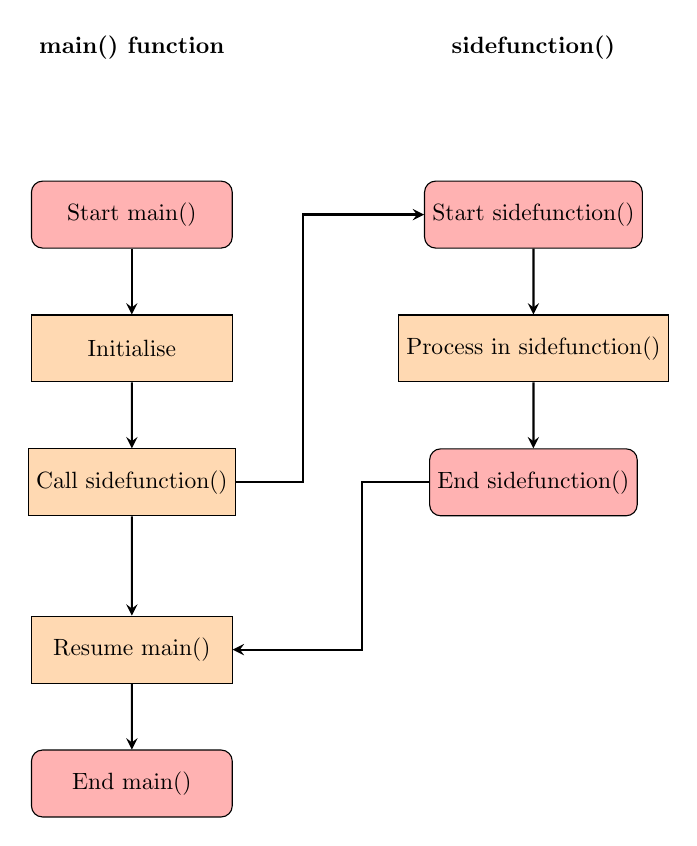
\begin{tikzpicture}[node distance=2cm, scale=0.85, transform shape]
		
		% Nodes for main function
		\node (start) [startstop] {Start main()};
		\node (init) [process, below of=start] {Initialise};
		\node (callsidefunction) [process, below of=init] {Call sidefunction()};
		\node (resume) [process, below of=callsidefunction, yshift=-0.5cm] {Resume main()};
		\node (end) [startstop, below of=resume] {End main()};
		
		% Nodes for sidefunction
		\node (startsidefunction) [startstop, right of=callsidefunction, xshift=4cm, yshift=4cm] {Start sidefunction()};
		\node (processsidefunction) [process, below of=startsidefunction] {Process in sidefunction()};
		\node (endsidefunction) [startstop, below of=processsidefunction] {End sidefunction()};
		
		% Arrows for main function
		\draw [arrow] (start) -- (init);
		\draw [arrow] (init) -- (callsidefunction);
		\draw [arrow] (callsidefunction) -- (resume);
		\draw [arrow] (resume) -- (end);
		
		% Arrows for sidefunction
		\draw [arrow] (startsidefunction) -- (processsidefunction);
		\draw [arrow] (processsidefunction) -- (endsidefunction);
		
		% Interprocedural arrows
		\draw [arrow] (callsidefunction.east) -- ++(1,0) |- (startsidefunction);
		\draw [arrow] (endsidefunction.west) -- ++(-1,0) |- (resume);
		
		% Labels
		\node [above of=start, yshift=0.5cm, text centered] {\textbf{main() function}};
		\node [above of=startsidefunction, yshift=0.5cm, xshift=0cm, text centered] {\textbf{sidefunction()}};
		
	\end{tikzpicture}
	\caption{Example of Inter-Procedural Control Flow Graph}
\end{figure}
In Figure 2.2, a simple ICFG is shown. There are two separate linear control flow graphs where the main function calls the sidefunction in its execution. To interpret the flow of the programme correctly, you need to consider the execution of sidefunction() and where it's called. The ICFG combines the two separate CFGs to ensure correct analysis.

There are multiple techniques to reduce the graph, such as node merging, edge contraction, and the elimination of non-important nodes, without losing any information required for the analysis and reducing the complexity of the RICFG. The reduction of the ICFG makes the analysis of large and complex software a lot more efficient. By minimising the amount of data while retaining enough detail, RICFGs are great for static analysis of data races \cite{wang2020}.

Node merging is combining nodes that represent redundant control flow paths to reduce the number of nodes in the graph. Edge contraction is simplifying the graph by reducing the number of edges between nodes. It collapses edges, that do not significantly affect the control flow of the graph. \cite{muchnick1997} The elimination of nodes is the main tool used in this work to reduce the CFG. Eliminating nodes that do not carry any essential information for the applied data analysis significantly reduces the amount of data the algorithm has to analyze. Overall, these techniques enhance the scalability of static analysis and make it more practical to analyse more complex data \cite{wang2020}.

\begin{figure}[H]
	\centering
	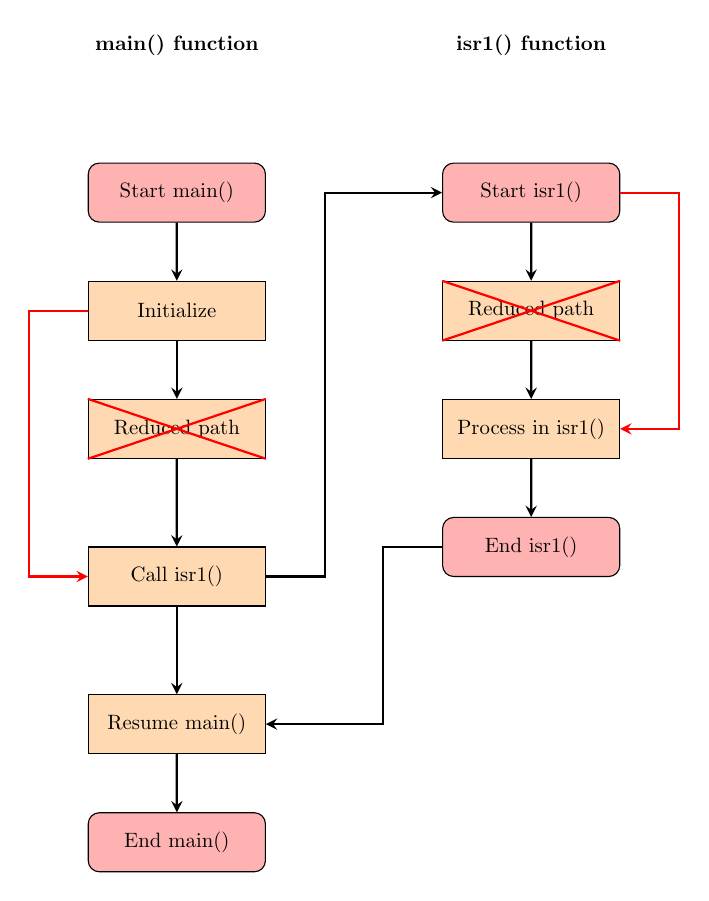
\begin{tikzpicture}[node distance=2cm, scale=0.75, transform shape]
		
		% Nodes for main function
		\node (start) [startstop] {Start main()};
		\node (init) [process, below of=start] {Initialize};
		\node (unimportant_main) [process, below of=init] {Reduced path};
		\node (callisr1) [process, below of=unimportant_main, yshift=-0.5cm] {Call isr1()};
		\node (resume) [process, below of=callisr1, yshift=-0.5cm] {Resume main()};
		\node (end) [startstop, below of=resume] {End main()};
		
		% Nodes for isr1 function
		\node (startisr1) [startstop, right of=callisr1, xshift=4cm, yshift=6.5cm] {Start isr1()};
		\node (unimportant_isr1) [process, below of=startisr1] {Reduced path};
		\node (processisr1) [process, below of=unimportant_isr1] {Process in isr1()};
		\node (endisr1) [startstop, below of=processisr1] {End isr1()};
		
		% Arrows for main function
		\draw [arrow] (start) -- (init);
		\draw [arrow] (init) -- (unimportant_main);
		\draw [arrow] (unimportant_main) -- (callisr1);
		\draw [arrow] (callisr1) -- (resume);
		\draw [arrow] (resume) -- (end);
		
		% Arrows for isr1 function
		\draw [arrow] (startisr1) -- (unimportant_isr1);
		\draw [arrow] (unimportant_isr1) -- (processisr1);
		\draw [arrow] (processisr1) -- (endisr1);
		
		% Interprocedural arrows
		\draw [arrow] (callisr1.east) -- ++(1,0) |- (startisr1);
		\draw [arrow] (endisr1.west) -- ++(-1,0) |- (resume);
		
		% Red arrows bypassing unimportant information
		\draw [redarrow] (init.west) -- ++(-1,0) |- (callisr1.west);
		\draw [redarrow] (startisr1.east) -- ++(1,0) |- (processisr1.east);
		
		% Red crosses over unimportant information
		\draw[red,thick] (unimportant_main.north west) -- (unimportant_main.south east);
		\draw[red,thick] (unimportant_main.north east) -- (unimportant_main.south west);
		\draw[red,thick] (unimportant_isr1.north west) -- (unimportant_isr1.south east);
		\draw[red,thick] (unimportant_isr1.north east) -- (unimportant_isr1.south west);
		
		% Labels
		\node [above of=start, yshift=0.5cm, text centered] {\textbf{main() function}};
		\node [above of=startisr1, yshift=0.5cm, xshift=0cm, text centered] {\textbf{isr1() function}};
		
	\end{tikzpicture}
	\caption{Example of Reduced Inter-Procedural Control Flow Graph}
\end{figure}

Figure 2.3 shows an example of a simple reduction by eliminating nodes that do not carry any important information for the analysis the RICFG is used for. 

\section{Data Races}

A data race occurs when two or more functions or threads access a shared resource concurrently, without being ordered by a happens-before relationship, and one of those accesses is a write operation \cite{chen2011}. This can lead to unpredictable behaviour and errors in the system, which makes the detection of data races a critical aspect of concurrent programmes.
Without proper synchronisation, a system with multiple threads or functions that use shared data will lead to data races. The outcome of a programme with data races is non-deterministic \cite{chen2011}. The order of execution of operations can vary, which may result in the generation of bugs that are not reproducible or difficult to reproduce. 
\begin{figure}[H]
	\centering
	\begin{algorithm}[H]
		\caption{Data Race Example}
		\KwData{long shared1;}
		
		\BlankLine
		\SetKwFunction{FMain}{main}
		\SetKwProg{Fn}{Function}{:}{}
		\Fn{\FMain()}{
			\BlankLine
			\textbf{Variables}:\\
			unsigned char tmp\;
			\BlankLine
			\textbf{Code}:\\
			tmp $\leftarrow$ shared1\;
		}
		
		\BlankLine
		\SetKwFunction{FIsr}{isr1}
		\Fn{\FIsr()}{
			\BlankLine
			\textbf{Code}:\\
			idlerun()\;
			shared1 $\leftarrow$ 1\;
			idlerun()\;
		}
	\end{algorithm}
	\caption{Simple Example of a Data Race}
\end{figure}

In Figure 2.4, an example of a simple data race is shown. A global variable shared1 is initiated and accessed in two different functions main() and isr1 (). Since there are no synchronisation tools used and the operation in isr1 is a write, there is a data race between line 5 and line 9.


\subsection{Detection Techniques}

Data race detection can be approached by two different analytical methods. Each of those methods provides benefits and challenges.

\subsubsection{Static Data Race Detection \cite{wang2020}}
\textbf{Advantages:}
\begin{itemize}
	\item Comprehensivness: Static analysis inspects the code without executing the programme by analysing every possible execution path and interactions that could lead to data races. 
	\item Early Detection: Since static analysis does not require execution, it can analyse the code in the development phase, allowing the developer to find issues without deployment.
\end{itemize}
\textbf{Disadvantages:}
\begin{itemize}
	\item False Positives/Negatives: Static analysis reports all data races that fall under certain conditions. Some of these data races could be very unlikely or even impossible at runtime. On the other hand, due to the approximations and assumptions necessary for tractability, it may miss some races.
	\item Complexity in Handling Dynamic Behaviour: Dynamic behaviours such as pointers or recursion can be challenging to analyse for static approaches, leading to incomplete or inaccurate results.
\end{itemize}

\subsubsection{Dynamic Data Race Detection \cite{flanagan2009}}
\textbf{Advantages:}
\begin{itemize}
	\item Precision: Dynamic analysis tools monitor the actual execution of a programme, identifying data races in real-time. Which results in reducing the number of false positives.
	\item Context-Sensitive Detection: By analysing the actual runtime behaviour, dynamic analysis can understand the context of operations, leading to more accurate detection. 
\end{itemize}
\textbf{Disadvantages:}
\begin{itemize}
	\item Performance Overhead: The analysis in runtime can slow down the application significantly. 
	\item Coverage: The effectiveness is heavily dependent on the execution path triggered during the tests. If certain parts of the programme are not passed through in the execution run, they are not analysed.
\end{itemize}

Both static and dynamic analysis are crucial for a complete analysis of a code. They complement each other's limitations. A combination of both is the best approach to detecting data races most reliable. However, in this work, I am going to focus on the static analysis of data races.


\subsection{Strategies for Preventing Data Races}

Preventing data races requires careful design and implementation of concurrent programs. One effective strategy is to use proper synchronisation mechanisms, such as mutexes, semaphores, and condition variables, to control access to shared data. These mechanisms ensure that only one thread can access the shared data at a time, preventing conflicting operations. Avoiding shared mutable states is another effective strategy, where threads operate on local copies of data instead of shared data, reducing the potential for conflicts. Designing thread-safe data structures and algorithms that inherently manage concurrent access also helps prevent data races, ensuring reliable and predictable programme behaviour \cite{herlihy2008}.

Preventing data races requires careful design and implementation of concurrent programs. Effective strategies for general prevention of data races are synchronisation mechanisms such as mutexes, semaphors, and condition variables, which control access to shared data. Those mechanisms ensure that only one thread can access the shared resource at a time \cite{herlihy2008}. Since I am focusing on data races in interrupt driven systems, the main tool to prevent data races is to disable ISRs, which access shared resources in critical areas.
\begin{figure}[H]
	\centering
	\begin{algorithm}[H]
		\caption{Enable/Disable ISR Call Example}
		\KwData{long shared1}
		
		\SetKwFunction{FMain}{main}
		\SetKwProg{Fn}{Function}{:}{}
		
		\Fn{\textbf{main()}}{
			\textbf{Variables}:\\
			unsigned char tmp\;
			\BlankLine
			\textbf{Code}:\\
			disable\_isr(1)\;
			tmp $\leftarrow$ shared1\;
			enable\_isr(1)\;
		}
		
		\Fn{\textbf{isr1()}}{
			\textbf{Code}:\\
			idlerun()\;
			shared1 $\leftarrow$ 1\;
			idlerun()\;
		}
		
		\Fn{\textbf{isr2()}}{
			\textbf{Code}:\\
			idlerun()\;
			int variable1 = 1\;
			idlerun()\;
		}
	\end{algorithm}
	\caption{Example of a Data Race with Enable/Disable ISR Calls}
\end{figure}
Figure 2.5 is an example of a disable ISR call that leads to the save access of the shared data. The main function and isr1 both access the shared resource shared1. Since the read operation in line 6 of the main function is safely accessed by disabling isr1 in line 5 and enabling it in line 7, a possible data race is prevented.
\section{Static Detection of Data Races in Interrupt-Driven Systems}

The asynchronous nature and concurrent execution of ISRs and the main function introduces significant challenges for data consistency and detecting data races in interrupt-driven systems. Static data race analysis, especially those using RICFGs, are a promising approach to identifying data races without the need for extensive testing and runtime monitoring as in dynamic approaches \cite{wang2020}.

The static approach involves the construction of an RICFG for the programme, which includes both the main code and ISRs, and capturing the control flow and potential interaction between them. Analysing the RICFG, shows paths where shared resources are accessed concurrently without proper synchronisation and indicates potential data races. Integrating the static analysis tool with the development process enables continuous detection of data races during software development, improving the reliability and correctness of interrupt-driven systems \cite{wang2020}.

The methodology for static data race detection in interrupt-driven systems involves the following key steps. First, the RICFGs are constructed for the entire programme, including the main code and the ISRs. This involves analysing the control flow and identifying interactions between the main programme and ISRs. Next, the RICFGs are analysed to find potential data races, focusing on paths where concurrent access of shared data is done without proper synchronization. Finally, the developer can use the analysis results to address identified data races in early development processes \cite{wang2020}.

\begin{figure}[H]
	\begin{algorithm}[H]
		\caption{Static Race Detection}
		\KwIn{RICFGs of P}
		\KwOut{potential racing pairs (PR)}
		
		\BlankLine
		\For{each $< G_i ; G_j >$ in RICFGs}{
			\For{each $sv_i \in G_i$}{
				\For{each $sv_j \in G_j$}{
					\If{$sv_i.V == sv_j.V$ and $(sv_i.A == W$ or $sv_j.A == W)$ and $G_i.pri < G_j.pri$ and $INTB.get(svi).contains(Gj)$}{
						$PR = PR \cup \{ <sv_i, sv_j> \}$\;
					}
				}
			}
		}
	\end{algorithm}
	\caption{Static Race Detection Approach by \cite{wang2020}}
\end{figure}

The approach by Wang et al. shows a computation of potential data races using RICFGs. By running a depth-first search on the RICFGs it finds the interrupt status of every instruction. If there is a shared resource in both of the analysed RICFGs, at least one of them is a write operation, and the two functions differ in their priority. While the interrupt in this pair is enabled, the two accesses are a potential data race \cite{wang2020}.
In the following, I am going to introduce you to the implementation of my static analysis programme based on the static race detection approach of Wang et al..


\chapter{Implementation}
In the following I will provide an indepth explanation of my implemenation. For the generation of the input I used GCC. The command \texttt{gcc -fdump-tree-cfg} provides a cfg-file with all important informations for the intended data race analysis. I have split the explanation of the implementation into the initialization of the basic block class, the parsing of the input, the actual data race analysis and the filter of false positives found in data race analysis.
\subsection*{Class BasicBlock}
\begin{algorithm}[H]
	\caption{BasicBlock Class Definition}
	\DontPrintSemicolon
	\SetAlgoLined
	
	\textbf{Class BasicBlock}:\\
	\Indp
	\textbf{Def} \_\_init\_\_(self, function\_name, number, shared\_resources, successors, enable\_disable\_calls, code):\\
	self.function\_name $\gets$ function\_name\;
	self.number $\gets$ number\;
	self.shared\_resources $\gets$ shared\_resources\;
	self.successors $\gets$ successors\;
	self.enable\_disable\_calls $\gets$ enable\_disable\_calls\;
	self.code $\gets$ code\;
	\Indm
\end{algorithm}

The class \texttt{BasicBlock} is a display of all the information nessessary for the data race analysis found in the input. Those informations include the following attributes:
\begin{itemize}
	\item \texttt{function\_name}: The function name to which the basic block belongs. 
	\item \texttt{number}: The number of the basic block.
	\item \texttt{shared\_resources}: All accesses of shared resources within the basic block. The access type (read/write) and also the line number of such calls are saved.
	\item \texttt{successors}: A list of all the successors of each basic block. Important to build all possible paths through the CFG.
	\item \texttt{enable\_disable\_calls}: All calls that disable or enable an ISR within this basic block and also with the corrsponding line number of those calls to ensure correct order.
	\item \texttt{code}: The lines of code of the block stored with their line number.
\end{itemize}


\subsection*{Parsing}
\begin{algorithm}[H]
	\caption{Parse Basic Blocks}
	\DontPrintSemicolon
	\SetAlgoLined
	\KwData{file\_path, shared\_resource\_names}
	\KwResult{Dictionary of BasicBlocks mapping (function name, block number) to BasicBlock instances}
	blocks $\gets$ empty dictionary\;
	current\_function $\gets$ None\;
	\SetKwInOut{Input}{input}\SetKwInOut{Output}{output}
	\KwIn{Path to source file, list of shared resource names}
	\KwOut{Dictionary of basic blocks with details}
	\BlankLine
	\For{each line in file at file\_path}{
		line $\gets$ line.strip()\;
		Increment line\_number\;
		\If{line starts new function}{
			\If{current block is open}{
				Save current block to blocks\;
			}
			Update current\_function and reset current block details\;
		}
		\ElseIf{line starts new basic block}{
			\If{current block is open}{
				Save current block to blocks\;
			}
			Initialize new block details\;
		}
		Update shared\_resources and enable\_disable\_calls based on line content\;
	}
	\If{current block is open at end of file}{
		Save last block to blocks\;
	}
	\ForEach{line indicating successor blocks}{
		Parse successor details and update block information in blocks\;
	}
	\Return{blocks}
\end{algorithm}

The function \texttt{parse\_basic\_blocks} starts with the initialisation of a dictionary \texttt{blocks} and a variable \texttt{current\_function}. It opens the file and reads its lines into a list \texttt{lines}.

These variables are initialised to collect information on basic blocks: 
\begin{itemize}
	\item \texttt{bb\_num}: Number of the current basic block.
	\item \texttt{shared\_resources}: List of shared resources in the current block.
	\item \texttt{enable\_disable\_calls}: List of ISR activation/deactivation calls.
	\item \texttt{code\_lines}: The lines of code of the current block.
	\item \texttt{line\_number}: The current line number in the file.
\end{itemize}


The loop runs through each line of the file, removes leading and trailing spaces and increments the line number. If a new function is recognised (by the pattern \texttt{;; Function ... (}), the current block is saved and the current function is updated.

If a new basic block number is detected (\texttt{<bb \(\d+\)>:}), the previous block is saved and the information for the new block is initialised.

This section searches each line for shared resources and ISR activation/deactivation calls. Resources and calls found are added to the corresponding list and the current line is added to \texttt{code\_lines}.

At the end of the loop, the last basic block is saved if there is still an open block.

In a second pass through the lines, the successor blocks for each basic block are identified and linked accordingly. Finally, the function returns the \texttt{blocks} dictionary.

\begin{algorithm}[H]
	\caption{Track ISR Status}
	\DontPrintSemicolon
	\SetAlgoLined
	\KwData{blocks}
	\KwResult{List indicating ISR status initialized to zero}
	\SetKwInOut{Input}{input}\SetKwInOut{Output}{output}
	\KwIn{Dictionary of BasicBlocks}
	\KwOut{List of zeros representing the status of each ISR}
	\BlankLine
	isr\_count $\gets$ count unique ISRs in function names from blocks\;
	\Return{list initialized to zero of length isr\_count}
\end{algorithm}

The function \texttt{track\_isr\_status} initialises the tracking of the ISR status. It returns a list of zeros whose length corresponds to the number of unique ISRs in the programme. This list is used to track the activation/deactivation status of each ISR.

\begin{algorithm}[H]
	\caption{Extract ISR Index}
	\DontPrintSemicolon
	\SetAlgoLined
	\KwData{function\_name}
	\KwResult{Zero-based index of the ISR or None if no ISR is found}
	\SetKwInOut{Input}{input}\SetKwInOut{Output}{output}
	\KwIn{Function name as a string}
	\KwOut{Integer index or None}
	\BlankLine
	match $\gets$ search for pattern 'isr[\_]?(\d+)' in function\_name\;
	\eIf{match is found}{
		\Return{integer value of the first group in match minus one}\;
	}{
		\Return{None}\;
	}
\end{algorithm}

The function \texttt{extract\_isr\_index} extracts the index of an ISR from a function name that follows the pattern \texttt{isr\_\d+}. It returns the index of the ISR reduced by one to enable zero-based indexing.

\subsection*{Data Race Detection}
The following functions are used to determine all possible data races which are filtered later in the code. The intention of this is to find all possible data races to minimize the amount of false negatives. Since false positives can be evaluated later by interpreting the output.

\begin{algorithm}[H]
	\caption{Initialization and ISR Enabling Map}
	\DontPrintSemicolon
	\SetAlgoLined
	\KwData{blocks}
	\KwResult{List of potential data races identified}
	\SetKwInOut{Input}{input}\SetKwInOut{Output}{output}
	\KwIn{Dictionary of BasicBlocks}
	\KwOut{List of potential data races}
	\BlankLine
	potential\_data\_races $\gets$ empty list\;
	resource\_accesses $\gets$ initialize as a default dictionary to list\;
	isr\_enabling\_map $\gets$ initialize as a default dictionary to set\;
	\BlankLine
	\ForEach{block in blocks}{
		\ForEach{call, line\_number in block.enable\_disable\_calls}{
			\If{call contains 'enable\_isr'}{
				isr\_idx\_match $\gets$ search for pattern '\(\d+\)' in call\;
				\If{isr\_idx\_match is found}{
					enabled\_isr\_idx $\gets$ integer value of the first group in isr\_idx\_match minus one\;
					enabler\_isr $\gets$ block.function\_name\;
					isr\_enabling\_map[enabler\_isr].add(enabled\_isr\_idx)\;
				}
			}
		}
	}
\end{algorithm}


The first part of the function \texttt{detect\_data\_races} takes a list of all basic block items as input. It also initializes the empty list of \texttt{potential\_data\_races}, a dictionary for \texttt{resource\_access} and a dictionary for the \texttt{isr\_enabling\_map}. \texttt{Potential\_data\_races} and \texttt{resource\_access} are used later in the code. The main loop of the function iterates through every item in blocks and finds basic blocks with \texttt{enable\_disable\_calls}. If there is an enable call in a block item, the index of the enabled ISR gets read and the basic block gets added to the \texttt{isr\_enabling\_map} with the information which ISR it enables.

\begin{algorithm}[H]
	\caption{Process Block}
	\DontPrintSemicolon
	\SetAlgoLined
	\KwData{block, current\_isr\_status}
	\KwResult{Updated ISR status and recorded resource accesses}
	\SetKwInOut{Input}{input}\SetKwInOut{Output}{output}
	\KwIn{A code block and the current ISR status as a list}
	\KwOut{Updated current ISR status and appended resource accesses to a global list}
	\BlankLine
	\ForEach{line, line\_number in block.code}{
		\If{line contains 'enable\_isr' or 'disable\_isr'}{
			isr\_idx\_match $\gets$ search for pattern '\(\d+\)' in line\;
			\If{isr\_idx\_match is found}{
				isr\_idx $\gets$ integer value of the first group in isr\_idx\_match minus one\;
				\eIf{"disable\_isr" is in line}{
					\If{0 $\leq$ isr\_idx $<$ length of current\_isr\_status}{
						current\_isr\_status[isr\_idx] $\gets$ 1\;  % Assuming 1 indicates disabled
					}
				}{
					\If{0 $\leq$ isr\_idx $<$ length of current\_isr\_status}{
						current\_isr\_status[isr\_idx] $\gets$ 0\;  % Assuming 0 indicates enabled
					}
				}
			}
		}
		\ForEach{resource\_name, access\_type, res\_line\_number in block.shared\_resources}{
			\If{res\_line\_number == line\_number}{
				resource\_accesses[resource\_name].append((block.function\_name, block.number, access\_type, line\_number, current\_isr\_status.copy()))\;
			}
		}
	}
\end{algorithm}


This part of the code runs thorugh each line of an basic block to find the current ISR status while resources get accessed. When a resource is found all the informations are added to the \texttt{resource\_accesses} dictionary which include the function name and the block number of the current basic block aswell as the access type, the line number and the ISR status of the access. All those informations are used later for the detection of the data races.

\begin{algorithm}[H]
	\caption{Depth-First Search (DFS) for Blocks}
	\DontPrintSemicolon
	\SetAlgoLined
	\KwData{block, visited\_blocks, current\_isr\_status, path}
	\KwResult{Recursive processing of blocks and their successors}
	\SetKwInOut{Input}{input}\SetKwInOut{Output}{output}
	\KwIn{A block, set of visited blocks, current ISR status, and path tracing the blocks visited}
	\KwOut{Processed blocks with updated ISR statuses and path}
	\BlankLine
	\If{(block.function\_name, block.number) is in visited\_blocks}{
		\Return  % Stop processing if the block has been visited
	}
	\BlankLine
	visited\_blocks.add((block.function\_name, block.number))\;  % Mark the block as visited
	path.append((block.function\_name, block.number))\;  % Add the block to the path
	\BlankLine
	process\_block(block, current\_isr\_status)\;  % Process the current block
	\BlankLine
	\If{block has successors}{
		\ForEach{successor in block.successors}{
			dfs(successor, set(visited\_blocks), current\_isr\_status.copy(), path.copy())\;  % Recursive call for each successor
		}
	}
\end{algorithm}

The \texttt{Depth-First Search (DFS)} function is recursively processing each block in a possible path of the RICFG. 

\begin{algorithm}[H]
	\caption{Initial Processing and Recursive Depth-First Search}
	\DontPrintSemicolon
	\SetAlgoLined
	\KwData{blocks (a dictionary of blocks indexed by function name and block number)}
	\KwResult{Executes process block and DFS on selected blocks and their successors}
	
	\BlankLine
	\ForEach{(func\_name, bb\_num) and block in blocks}{
		\If{bb\_num = 2}{
			initial\_isr\_status $\gets$ track\_isr\_status(blocks)\;
			process\_block(block, initial\_isr\_status)\;
			\ForEach{successor in block.successors}{
				dfs(successor, \{\}, initial\_isr\_status.copy(), [(func\_name, bb\_num)])\;
			}
		}
	}
\end{algorithm}


This section initialises the depth search for basic blocks with the number 2 and starts processing and running through the successor blocks.

\begin{algorithm}[H]
	\caption{Check for Data Races}
	\DontPrintSemicolon
	\SetAlgoLined
	\KwResult{Update global list of potential data races based on access patterns}
	\SetKwInOut{Output}{output}
	\KwOut{Updated list of potential data races with detailed conflict info}
	\BlankLine
	\ForEach{resource, accesses in resource\_accesses}{
		\For{i $\gets$ 0 \KwTo length(accesses)-1}{
			func1, bb\_num1, access\_type1, line\_number1, isr\_status1 $\gets$ accesses[i]\;
			\For{j $\gets$ i+1 \KwTo length(accesses)-1}{
				func2, bb\_num2, access\_type2, line\_number2, isr\_status2 $\gets$ accesses[j]\;
				\If{func1 $\neq$ func2 and (access\_type1 = "write" or access\_type2 = "write")}{
					potential\_data\_races.append((resource, (func1, bb\_num1, access\_type1, line\_number1, isr\_status1), (func2, bb\_num2, access\_type2, line\_number2, isr\_status2)))\;
				}
			}
		}
	}
\end{algorithm}

The function \texttt{check\_for\_data\_races} identifies potential data races by comparing pairs of resource accesses. If two accesses to the same resource originate from different functions and at least one of them is a write access, a potential data race is identified.


Calling \texttt{check\_for\_data\_races} performs a check of the potential data races.
\subsection*{Filter Possible Data Races}
\begin{algorithm}[H]
	\caption{Filter Data Races}
	\DontPrintSemicolon
	\SetAlgoLined
	\KwData{potential\_data\_races}
	\KwResult{Filtered list of data races}
	
	\SetKwFunction{FMain}{filter\_data\_races}
	\SetKwFunction{FSubOne}{is\_isr\_disabled}
	\SetKwFunction{FSubTwo}{is\_isr\_enabled\_by\_another}
	\SetKwProg{Fn}{Function}{:}{end}
	
	\Fn{\FMain{potential\_data\_races}}{
		filtered\_data\_races $\gets$ empty list\;
		\ForEach{resource, access1, access2 in potential\_data\_races}{
			Decompose access1 into func1, bb\_num1, access\_type1, line\_number1, isr\_status1\;
			Decompose access2 into func2, bb\_num2, access\_type2, line\_number2, isr\_status2\;
			
			relevant\_isr\_disabled1 $\gets$ \FSubOne{isr\_status1, func2} and not \FSubTwo{isr\_status1, func2}\;
			relevant\_isr\_disabled2 $\gets$ \FSubOne{isr\_status2, func1} and not \FSubTwo{isr\_status2, func1}\;
			
			\If{not (relevant\_isr\_disabled1 or relevant\_isr\_disabled2)}{
				filtered\_data\_races.append((resource, access1, access2))\;
			}
		}
		\Return{filtered\_data\_races}\;
	}
	
	\Fn{\FSubOne{isr\_status, func\_name}}{
		isr\_idx $\gets$ extract\_isr\_index(func\_name)\;
		\If{isr\_idx is not None and isr\_idx $<$ length of isr\_status}{
			\Return{isr\_status[isr\_idx] == 1}\; \tcp{1 indicates disabled}
		}
		\Return{False}\;
	}
	
	\Fn{\FSubTwo{isr\_status, func\_name}}{
		isr\_idx $\gets$ extract\_isr\_index(func\_name)\;
		\If{isr\_idx is not None}{
			\ForEach{enabler\_isr, enabled\_isrs in isr\_enabling\_map}{
				enabler\_idx $\gets$ extract\_isr\_index(enabler\_isr)\;
				\If{enabler\_idx is not None and not \FSubOne{isr\_status, enabler\_isr}}{
					\If{isr\_idx in enabled\_isrs}{
						\Return{True}\;
					}
				}
			}
		}
		\Return{False}\;
	}
\end{algorithm}

The function \texttt{filter\_data\_races} filters false positives from the list of potential data races. It checks the ISR status during resource accesses and only confirms data races if relevant ISRs were not deactivated at access time or activated by another function. At the end, \texttt{detect\_data\_races} returns the filtered data races.


\chapter{Evaluation}
1,5 Woche 
\chapter{Conclusion}
Indroduction+Conclusion und Allgemeine Überarbeitung 0,5 Woche
1 Wochen Korrekturlesen und Einarbeitung
=9 Wochen bei Vollarbeitszeit an BE
\appendix
}
\backmatter{}
\chapter{Bibliography}
Lightweight Data Race Detection for Production by Swarnendu Biswas, Man Cao, Minjia Zhang, Michael D. Bond, Benjamin P. Wood


A Deployable Sampling Strategy for Data Race Detection by Yan Cai1, Jian Zhang, Lingwei Cao, and Jian Liu
\begin{thebibliography}{9}
	\bibitem{wang2020}
	Wang, Y., Gao, F., Wang, L., Yu, T., Zhao, J., \& Li, X. (2020). Automatic Detection, Validation, and Repair of Race Conditions in Interrupt-Driven Embedded Software. IEEE Transactions on Software Engineering.
	
	\bibitem{engler2003}
	Engler, D., \& Ashcraft, K. (2003). RacerX: Effective, Static Detection of Race Conditions and Deadlocks. ACM SIGOPS Operating Systems Review.
	
	\bibitem{chopra2019}
	Nikita Chopra, Rekha Pai, and Deepak D’Souza (2019). Data Races and Static Analysis for Interrupt-Driven Kernels
	
	\bibitem{flanagan2009}
	Flanagan, C., \& Freund, S. N. (2009). FastTrack: Efficient and Precise Dynamic Race Detection. ACM SIGPLAN Notices.
	
	\bibitem{chen2011}
	R. Chen, Xiangying Guo, Y. Duan, B. Gu, Mengfei Yang (2011). Static Data Race Detection for Interrupt-Driven Embedded Software.
			
	\bibitem{muchnick1997}
	Muchnick, S. S. (1997). Advanced Compiler Design and Implementation. Morgan Kaufmann.
	
	\bibitem{adve1996}
	Adve, S. V., \& Gharachorloo, K. (1996). Shared Memory Consistency Models: A Tutorial. IEEE Computer.
	
	\bibitem{herlihy2008}
	Herlihy, M., \& Shavit, N. (2008). The Art of Multiprocessor Programming. Morgan Kaufmann.
\end{thebibliography}
\chapter{Attachments}
\begin{lstlisting}[language=Python, mathescape, escapeinside={(*}{*)}]
	class BasicBlock:
	def __init__(function_name, number, shared_resources=[], successors=[], enable_disable_calls=[], code=[]):
	self.function_name = function_name
	self.number = number
	self.shared_resources = shared_resources
	self.successors = successors
	self.enable_disable_calls = enable_disable_calls
	self.code = code
	
	def __repr__():
	return ("BasicBlock(function_name={}, number={}, shared_resources={}, "
	"successors={}, enable_disable_calls={}, code={})".format(
	self.function_name, self.number, self.shared_resources, 
	[succ.number for succ in self.successors], self.enable_disable_calls, 
	' '.join(self.code)))
	
	def parse_basic_blocks(file_path, shared_resource_names):
	blocks = {}
	current_function = None
	
	with open(file_path, 'r') as file:
	lines = file.readlines()
	
	bb_num = None
	shared_resources = []
	enable_disable_calls = []
	code_lines = []
	line_number = 0  
	
	for line in lines:
	line = line.strip()
	line_number += 1
	
	func_match = re.match(r';; Function (.+?) \(', line)
	if func_match:
	if bb_num is not None and current_function is not None:
	blocks[(current_function, bb_num)] = BasicBlock(
	current_function, bb_num, shared_resources, [], enable_disable_calls, code_lines)
	current_function = func_match.group(1)
	bb_num = None
	continue
	
	bb_match = re.match(r'<bb (\d+)>:', line)
	if bb_match:
	if bb_num is not None and current_function is not None:
	blocks[(current_function, bb_num)] = BasicBlock(
	current_function, bb_num, shared_resources, [], enable_disable_calls, code_lines)
	bb_num = int(bb_match.group(1))
	shared_resources = []
	enable_disable_calls = []
	code_lines = []
	
	for resource_name in shared_resource_names:
	if re.search(fr'\b{resource_name}\b', line):
	if re.search(fr'\b{resource_name}\b\s*=', line):
	shared_resources.append((resource_name, 'write', line_number))
	else:
	shared_resources.append((resource_name, 'read', line_number))
	
	if 'enable_isr' in line or 'disable_isr' in line:
	enable_disable_calls.append((line.strip(), line_number))
	
	code_lines.append((line, line_number))
	
	if bb_num is not None and current_function is not None:
	blocks[(current_function, bb_num)] = BasicBlock(
	current_function, bb_num, shared_resources, [], enable_disable_calls, code_lines)
	
	current_function = None
	bb_num = None
	for line in lines:
	line = line.strip()
	
	func_match = re.match(r';; Function (.+?) \(', line)
	if func_match:
	current_function = func_match.group(1)
	bb_num = None
	continue
	
	if 'succs' in line:
	succ_match = re.match(r';; (\d+) succs \{(.+?)\}', line)
	if succ_match:
	bb_num = int(succ_match.group(1))
	succ_list = [int(succ.strip()) for succ in succ_match.group(2).split()]
	if (current_function, bb_num) in blocks:
	blocks[(current_function, bb_num)].successors = [
	blocks[(current_function, succ)] for succ in succ_list if (current_function, succ) in blocks]
	
	return blocks
	
	def track_isr_status(blocks):
	isr_count = len(set(block.function_name for block in blocks.values() if re.search(r'isr[_]?\d+', block.function_name)))
	return [0] * isr_count  
	
	def extract_isr_index(function_name):
	match = re.search(r'isr[_]?(\d+)', function_name)
	if match:
	return int(match.group(1)) - 1
	return None
	
	def detect_data_races(blocks):
	potential_data_races = []
	resource_accesses = defaultdict(list)
	isr_enabling_map = defaultdict(set)
	
	for block in blocks.values():
	for call, line_number in block.enable_disable_calls:
	if 'enable_isr' in call:
	isr_idx_match = re.search(r'\((\d+)\)', call)
	if isr_idx_match:
	enabled_isr_idx = int(isr_idx_match.group(1)) - 1
	enabler_isr = block.function_name
	isr_enabling_map[enabler_isr].add(enabled_isr_idx)
	
	def process_block(block, current_isr_status):
	for line, line_number in block.code:
	if 'enable_isr' in line or 'disable_isr' in line:
	isr_idx_match = re.search(r'\((\d+)\)', line)
	if isr_idx_match:
	isr_idx = int(isr_idx_match.group(1)) - 1  
	if "disable_isr" in line:
	if 0 <= isr_idx < len(current_isr_status):
	current_isr_status[isr_idx] = 1
	elif "enable_isr" in line:
	if 0 <= isr_idx < len(current_isr_status):
	current_isr_status[isr_idx] = 0
	
	
	for resource_name, access_type, res_line_number in block.shared_resources:
	if res_line_number == line_number:
	resource_accesses[resource_name].append((block.function_name, block.number, access_type, line_number, current_isr_status.copy()))
	
	def dfs(block, visited_blocks, current_isr_status, path):
	if (block.function_name, block.number) in visited_blocks:
	return
	visited_blocks.add((block.function_name, block.number))
	path.append((block.function_name, block.number))
	
	process_block(block, current_isr_status)
	
	if not block.successors:
	pass
	else:
	for successor in block.successors:
	dfs(successor, set(visited_blocks), current_isr_status.copy(), path.copy())
	
	
	for (func_name, bb_num), block in blocks.items():
	if bb_num == 2:  
	initial_isr_status = track_isr_status(blocks).copy()
	process_block(block, initial_isr_status)
	for successor in block.successors:
	dfs(successor, set(), initial_isr_status.copy(), [(func_name, bb_num)])
	
	
	def check_for_data_races():
	for resource, accesses in resource_accesses.items():
	for i, (func1, bb_num1, access_type1, line_number1, isr_status1) in enumerate(accesses):
	for j, (func2, bb_num2, access_type2, line_number2, isr_status2) in enumerate(accesses):
	if i >= j:
	continue  
	if func1 != func2 and (access_type1 == "write" or access_type2 == "write"):
	potential_data_races.append((resource, (func1, bb_num1, access_type1, line_number1, isr_status1),
	(func2, bb_num2, access_type2, line_number2, isr_status2)))
	
	check_for_data_races()
	
	
	def filter_data_races(potential_data_races):
	filtered_data_races = []
	for resource, access1, access2 in potential_data_races:
	func1, bb_num1, access_type1, line_number1, isr_status1 = access1
	func2, bb_num2, access_type2, line_number2, isr_status2 = access2
	
	def is_isr_disabled(isr_status, func_name):
	isr_idx = extract_isr_index(func_name)
	if isr_idx is not None and isr_idx < len(isr_status):
	return isr_status[isr_idx] == 1
	return False
	
	def is_isr_enabled_by_another(isr_status, func_name):
	isr_idx = extract_isr_index(func_name)
	if isr_idx is not None:
	for enabler_isr, enabled_isrs in isr_enabling_map.items():
	enabler_idx = extract_isr_index(enabler_isr)
	if enabler_idx is not None and not is_isr_disabled(isr_status, enabler_isr):
	if isr_idx in enabled_isrs:
	return True
	return False
	
	relevant_isr_disabled1 = is_isr_disabled(isr_status1, func2) and not is_isr_enabled_by_another(isr_status1, func2)
	relevant_isr_disabled2 = is_isr_disabled(isr_status2, func1) and not is_isr_enabled_by_another(isr_status2, func1)
	
	if not (relevant_isr_disabled1 or relevant_isr_disabled2):
	filtered_data_races.append((resource, access1, access2))
	
	return filtered_data_races
	
	filtered_data_races = filter_data_races(potential_data_races)
	
	return filtered_data_races
	
	
	shared_resource_input = input("Enter the names of shared resources, separated by commas: ")
	shared_resource_names = [name.strip() for name in shared_resource_input.split(',')]
	
	file_path = input("Enter the file path: ").strip()
	blocks = parse_basic_blocks(file_path, shared_resource_names)
	
	data_races = detect_data_races(blocks)
	
	print("Detected Data Races:")
	for resource, access1, access2 in data_races:
	print(f"Resource: {resource}")
	print(f"  Access 1: Function {access1[0]} (BB {access1[1]}), {access1[2]}, Line {access1[3]}, ISR Status: {access1[4]}")
	print(f"  Access 2: Function {access2[0]} (BB {access2[1]}), {access2[2]}, Line {access2[3]}, ISR Status: {access2[4]}")
	print()
\end{lstlisting}
\end{document}